\documentclass[letterpaper]{article}
\usepackage[submission]{aaai2027}

%%%%% NEW MATH DEFINITIONS %%%%%

\usepackage{amsmath,amsfonts,bm}

% Mark sections of captions for referring to divisions of figures
\newcommand{\figleft}{{\em (Left)}}
\newcommand{\figcenter}{{\em (Center)}}
\newcommand{\figright}{{\em (Right)}}
\newcommand{\figtop}{{\em (Top)}}
\newcommand{\figbottom}{{\em (Bottom)}}
\newcommand{\captiona}{{\em (a)}}
\newcommand{\captionb}{{\em (b)}}
\newcommand{\captionc}{{\em (c)}}
\newcommand{\captiond}{{\em (d)}}

% Highlight a newly defined term
\newcommand{\newterm}[1]{{\bf #1}}


% Figure reference, lower-case.
\def\figref#1{figure~\ref{#1}}
% Figure reference, capital. For start of sentence
\def\Figref#1{Figure~\ref{#1}}
\def\twofigref#1#2{figures \ref{#1} and \ref{#2}}
\def\quadfigref#1#2#3#4{figures \ref{#1}, \ref{#2}, \ref{#3} and \ref{#4}}
% Section reference, lower-case.
\def\secref#1{section~\ref{#1}}
% Section reference, capital.
\def\Secref#1{Section~\ref{#1}}
% Reference to two sections.
\def\twosecrefs#1#2{sections \ref{#1} and \ref{#2}}
% Reference to three sections.
\def\secrefs#1#2#3{sections \ref{#1}, \ref{#2} and \ref{#3}}
% Reference to an equation, lower-case.
\def\eqref#1{equation~\ref{#1}}
% Reference to an equation, upper case
\def\Eqref#1{Equation~\ref{#1}}
% A raw reference to an equation---avoid using if possible
\def\plaineqref#1{\ref{#1}}
% Reference to a chapter, lower-case.
\def\chapref#1{chapter~\ref{#1}}
% Reference to an equation, upper case.
\def\Chapref#1{Chapter~\ref{#1}}
% Reference to a range of chapters
\def\rangechapref#1#2{chapters\ref{#1}--\ref{#2}}
% Reference to an algorithm, lower-case.
\def\algref#1{algorithm~\ref{#1}}
% Reference to an algorithm, upper case.
\def\Algref#1{Algorithm~\ref{#1}}
\def\twoalgref#1#2{algorithms \ref{#1} and \ref{#2}}
\def\Twoalgref#1#2{Algorithms \ref{#1} and \ref{#2}}
% Reference to a part, lower case
\def\partref#1{part~\ref{#1}}
% Reference to a part, upper case
\def\Partref#1{Part~\ref{#1}}
\def\twopartref#1#2{parts \ref{#1} and \ref{#2}}

\def\ceil#1{\lceil #1 \rceil}
\def\floor#1{\lfloor #1 \rfloor}
\def\1{\bm{1}}
\newcommand{\train}{\mathcal{D}}
\newcommand{\valid}{\mathcal{D_{\mathrm{valid}}}}
\newcommand{\test}{\mathcal{D_{\mathrm{test}}}}

\def\eps{{\epsilon}}


% Random variables
\def\reta{{\textnormal{$\eta$}}}
\def\ra{{\textnormal{a}}}
\def\rb{{\textnormal{b}}}
\def\rc{{\textnormal{c}}}
\def\rd{{\textnormal{d}}}
\def\re{{\textnormal{e}}}
\def\rf{{\textnormal{f}}}
\def\rg{{\textnormal{g}}}
\def\rh{{\textnormal{h}}}
\def\ri{{\textnormal{i}}}
\def\rj{{\textnormal{j}}}
\def\rk{{\textnormal{k}}}
\def\rl{{\textnormal{l}}}
% rm is already a command, just don't name any random variables m
\def\rn{{\textnormal{n}}}
\def\ro{{\textnormal{o}}}
\def\rp{{\textnormal{p}}}
\def\rq{{\textnormal{q}}}
\def\rr{{\textnormal{r}}}
\def\rs{{\textnormal{s}}}
\def\rt{{\textnormal{t}}}
\def\ru{{\textnormal{u}}}
\def\rv{{\textnormal{v}}}
\def\rw{{\textnormal{w}}}
\def\rx{{\textnormal{x}}}
\def\ry{{\textnormal{y}}}
\def\rz{{\textnormal{z}}}

% Random vectors
\def\rvepsilon{{\mathbf{\epsilon}}}
\def\rvtheta{{\mathbf{\theta}}}
\def\rva{{\mathbf{a}}}
\def\rvb{{\mathbf{b}}}
\def\rvc{{\mathbf{c}}}
\def\rvd{{\mathbf{d}}}
\def\rve{{\mathbf{e}}}
\def\rvf{{\mathbf{f}}}
\def\rvg{{\mathbf{g}}}
\def\rvh{{\mathbf{h}}}
\def\rvu{{\mathbf{i}}}
\def\rvj{{\mathbf{j}}}
\def\rvk{{\mathbf{k}}}
\def\rvl{{\mathbf{l}}}
\def\rvm{{\mathbf{m}}}
\def\rvn{{\mathbf{n}}}
\def\rvo{{\mathbf{o}}}
\def\rvp{{\mathbf{p}}}
\def\rvq{{\mathbf{q}}}
\def\rvr{{\mathbf{r}}}
\def\rvs{{\mathbf{s}}}
\def\rvt{{\mathbf{t}}}
\def\rvu{{\mathbf{u}}}
\def\rvv{{\mathbf{v}}}
\def\rvw{{\mathbf{w}}}
\def\rvx{{\mathbf{x}}}
\def\rvy{{\mathbf{y}}}
\def\rvz{{\mathbf{z}}}

% Elements of random vectors
\def\erva{{\textnormal{a}}}
\def\ervb{{\textnormal{b}}}
\def\ervc{{\textnormal{c}}}
\def\ervd{{\textnormal{d}}}
\def\erve{{\textnormal{e}}}
\def\ervf{{\textnormal{f}}}
\def\ervg{{\textnormal{g}}}
\def\ervh{{\textnormal{h}}}
\def\ervi{{\textnormal{i}}}
\def\ervj{{\textnormal{j}}}
\def\ervk{{\textnormal{k}}}
\def\ervl{{\textnormal{l}}}
\def\ervm{{\textnormal{m}}}
\def\ervn{{\textnormal{n}}}
\def\ervo{{\textnormal{o}}}
\def\ervp{{\textnormal{p}}}
\def\ervq{{\textnormal{q}}}
\def\ervr{{\textnormal{r}}}
\def\ervs{{\textnormal{s}}}
\def\ervt{{\textnormal{t}}}
\def\ervu{{\textnormal{u}}}
\def\ervv{{\textnormal{v}}}
\def\ervw{{\textnormal{w}}}
\def\ervx{{\textnormal{x}}}
\def\ervy{{\textnormal{y}}}
\def\ervz{{\textnormal{z}}}

% Random matrices
\def\rmA{{\mathbf{A}}}
\def\rmB{{\mathbf{B}}}
\def\rmC{{\mathbf{C}}}
\def\rmD{{\mathbf{D}}}
\def\rmE{{\mathbf{E}}}
\def\rmF{{\mathbf{F}}}
\def\rmG{{\mathbf{G}}}
\def\rmH{{\mathbf{H}}}
\def\rmI{{\mathbf{I}}}
\def\rmJ{{\mathbf{J}}}
\def\rmK{{\mathbf{K}}}
\def\rmL{{\mathbf{L}}}
\def\rmM{{\mathbf{M}}}
\def\rmN{{\mathbf{N}}}
\def\rmO{{\mathbf{O}}}
\def\rmP{{\mathbf{P}}}
\def\rmQ{{\mathbf{Q}}}
\def\rmR{{\mathbf{R}}}
\def\rmS{{\mathbf{S}}}
\def\rmT{{\mathbf{T}}}
\def\rmU{{\mathbf{U}}}
\def\rmV{{\mathbf{V}}}
\def\rmW{{\mathbf{W}}}
\def\rmX{{\mathbf{X}}}
\def\rmY{{\mathbf{Y}}}
\def\rmZ{{\mathbf{Z}}}

% Elements of random matrices
\def\ermA{{\textnormal{A}}}
\def\ermB{{\textnormal{B}}}
\def\ermC{{\textnormal{C}}}
\def\ermD{{\textnormal{D}}}
\def\ermE{{\textnormal{E}}}
\def\ermF{{\textnormal{F}}}
\def\ermG{{\textnormal{G}}}
\def\ermH{{\textnormal{H}}}
\def\ermI{{\textnormal{I}}}
\def\ermJ{{\textnormal{J}}}
\def\ermK{{\textnormal{K}}}
\def\ermL{{\textnormal{L}}}
\def\ermM{{\textnormal{M}}}
\def\ermN{{\textnormal{N}}}
\def\ermO{{\textnormal{O}}}
\def\ermP{{\textnormal{P}}}
\def\ermQ{{\textnormal{Q}}}
\def\ermR{{\textnormal{R}}}
\def\ermS{{\textnormal{S}}}
\def\ermT{{\textnormal{T}}}
\def\ermU{{\textnormal{U}}}
\def\ermV{{\textnormal{V}}}
\def\ermW{{\textnormal{W}}}
\def\ermX{{\textnormal{X}}}
\def\ermY{{\textnormal{Y}}}
\def\ermZ{{\textnormal{Z}}}

% Vectors
\def\vzero{{\bm{0}}}
\def\vone{{\bm{1}}}
\def\vmu{{\bm{\mu}}}
\def\vtheta{{\bm{\theta}}}
\def\va{{\bm{a}}}
\def\vb{{\bm{b}}}
\def\vc{{\bm{c}}}
\def\vd{{\bm{d}}}
\def\ve{{\bm{e}}}
\def\vf{{\bm{f}}}
\def\vg{{\bm{g}}}
\def\vh{{\bm{h}}}
\def\vi{{\bm{i}}}
\def\vj{{\bm{j}}}
\def\vk{{\bm{k}}}
\def\vl{{\bm{l}}}
\def\vm{{\bm{m}}}
\def\vn{{\bm{n}}}
\def\vo{{\bm{o}}}
\def\vp{{\bm{p}}}
\def\vq{{\bm{q}}}
\def\vr{{\bm{r}}}
\def\vs{{\bm{s}}}
\def\vt{{\bm{t}}}
\def\vu{{\bm{u}}}
\def\vv{{\bm{v}}}
\def\vw{{\bm{w}}}
\def\vx{{\bm{x}}}
\def\vy{{\bm{y}}}
\def\vz{{\bm{z}}}

% Elements of vectors
\def\evalpha{{\alpha}}
\def\evbeta{{\beta}}
\def\evepsilon{{\epsilon}}
\def\evlambda{{\lambda}}
\def\evomega{{\omega}}
\def\evmu{{\mu}}
\def\evpsi{{\psi}}
\def\evsigma{{\sigma}}
\def\evtheta{{\theta}}
\def\eva{{a}}
\def\evb{{b}}
\def\evc{{c}}
\def\evd{{d}}
\def\eve{{e}}
\def\evf{{f}}
\def\evg{{g}}
\def\evh{{h}}
\def\evi{{i}}
\def\evj{{j}}
\def\evk{{k}}
\def\evl{{l}}
\def\evm{{m}}
\def\evn{{n}}
\def\evo{{o}}
\def\evp{{p}}
\def\evq{{q}}
\def\evr{{r}}
\def\evs{{s}}
\def\evt{{t}}
\def\evu{{u}}
\def\evv{{v}}
\def\evw{{w}}
\def\evx{{x}}
\def\evy{{y}}
\def\evz{{z}}

% Matrix
\def\mA{{\bm{A}}}
\def\mB{{\bm{B}}}
\def\mC{{\bm{C}}}
\def\mD{{\bm{D}}}
\def\mE{{\bm{E}}}
\def\mF{{\bm{F}}}
\def\mG{{\bm{G}}}
\def\mH{{\bm{H}}}
\def\mI{{\bm{I}}}
\def\mJ{{\bm{J}}}
\def\mK{{\bm{K}}}
\def\mL{{\bm{L}}}
\def\mM{{\bm{M}}}
\def\mN{{\bm{N}}}
\def\mO{{\bm{O}}}
\def\mP{{\bm{P}}}
\def\mQ{{\bm{Q}}}
\def\mR{{\bm{R}}}
\def\mS{{\bm{S}}}
\def\mT{{\bm{T}}}
\def\mU{{\bm{U}}}
\def\mV{{\bm{V}}}
\def\mW{{\bm{W}}}
\def\mX{{\bm{X}}}
\def\mY{{\bm{Y}}}
\def\mZ{{\bm{Z}}}
\def\mBeta{{\bm{\beta}}}
\def\mPhi{{\bm{\Phi}}}
\def\mLambda{{\bm{\Lambda}}}
\def\mSigma{{\bm{\Sigma}}}

% Tensor
\DeclareMathAlphabet{\mathsfit}{\encodingdefault}{\sfdefault}{m}{sl}
\SetMathAlphabet{\mathsfit}{bold}{\encodingdefault}{\sfdefault}{bx}{n}
\newcommand{\tens}[1]{\bm{\mathsfit{#1}}}
\def\tA{{\tens{A}}}
\def\tB{{\tens{B}}}
\def\tC{{\tens{C}}}
\def\tD{{\tens{D}}}
\def\tE{{\tens{E}}}
\def\tF{{\tens{F}}}
\def\tG{{\tens{G}}}
\def\tH{{\tens{H}}}
\def\tI{{\tens{I}}}
\def\tJ{{\tens{J}}}
\def\tK{{\tens{K}}}
\def\tL{{\tens{L}}}
\def\tM{{\tens{M}}}
\def\tN{{\tens{N}}}
\def\tO{{\tens{O}}}
\def\tP{{\tens{P}}}
\def\tQ{{\tens{Q}}}
\def\tR{{\tens{R}}}
\def\tS{{\tens{S}}}
\def\tT{{\tens{T}}}
\def\tU{{\tens{U}}}
\def\tV{{\tens{V}}}
\def\tW{{\tens{W}}}
\def\tX{{\tens{X}}}
\def\tY{{\tens{Y}}}
\def\tZ{{\tens{Z}}}


% Graph
\def\gA{{\mathcal{A}}}
\def\gB{{\mathcal{B}}}
\def\gC{{\mathcal{C}}}
\def\gD{{\mathcal{D}}}
\def\gE{{\mathcal{E}}}
\def\gF{{\mathcal{F}}}
\def\gG{{\mathcal{G}}}
\def\gH{{\mathcal{H}}}
\def\gI{{\mathcal{I}}}
\def\gJ{{\mathcal{J}}}
\def\gK{{\mathcal{K}}}
\def\gL{{\mathcal{L}}}
\def\gM{{\mathcal{M}}}
\def\gN{{\mathcal{N}}}
\def\gO{{\mathcal{O}}}
\def\gP{{\mathcal{P}}}
\def\gQ{{\mathcal{Q}}}
\def\gR{{\mathcal{R}}}
\def\gS{{\mathcal{S}}}
\def\gT{{\mathcal{T}}}
\def\gU{{\mathcal{U}}}
\def\gV{{\mathcal{V}}}
\def\gW{{\mathcal{W}}}
\def\gX{{\mathcal{X}}}
\def\gY{{\mathcal{Y}}}
\def\gZ{{\mathcal{Z}}}

% Sets
\def\sA{{\mathbb{A}}}
\def\sB{{\mathbb{B}}}
\def\sC{{\mathbb{C}}}
\def\sD{{\mathbb{D}}}
% Don't use a set called E, because this would be the same as our symbol
% for expectation.
\def\sF{{\mathbb{F}}}
\def\sG{{\mathbb{G}}}
\def\sH{{\mathbb{H}}}
\def\sI{{\mathbb{I}}}
\def\sJ{{\mathbb{J}}}
\def\sK{{\mathbb{K}}}
\def\sL{{\mathbb{L}}}
\def\sM{{\mathbb{M}}}
\def\sN{{\mathbb{N}}}
\def\sO{{\mathbb{O}}}
\def\sP{{\mathbb{P}}}
\def\sQ{{\mathbb{Q}}}
\def\sR{{\mathbb{R}}}
\def\sS{{\mathbb{S}}}
\def\sT{{\mathbb{T}}}
\def\sU{{\mathbb{U}}}
\def\sV{{\mathbb{V}}}
\def\sW{{\mathbb{W}}}
\def\sX{{\mathbb{X}}}
\def\sY{{\mathbb{Y}}}
\def\sZ{{\mathbb{Z}}}

% Entries of a matrix
\def\emLambda{{\Lambda}}
\def\emA{{A}}
\def\emB{{B}}
\def\emC{{C}}
\def\emD{{D}}
\def\emE{{E}}
\def\emF{{F}}
\def\emG{{G}}
\def\emH{{H}}
\def\emI{{I}}
\def\emJ{{J}}
\def\emK{{K}}
\def\emL{{L}}
\def\emM{{M}}
\def\emN{{N}}
\def\emO{{O}}
\def\emP{{P}}
\def\emQ{{Q}}
\def\emR{{R}}
\def\emS{{S}}
\def\emT{{T}}
\def\emU{{U}}
\def\emV{{V}}
\def\emW{{W}}
\def\emX{{X}}
\def\emY{{Y}}
\def\emZ{{Z}}
\def\emSigma{{\Sigma}}

% entries of a tensor
% Same font as tensor, without \bm wrapper
\newcommand{\etens}[1]{\mathsfit{#1}}
\def\etLambda{{\etens{\Lambda}}}
\def\etA{{\etens{A}}}
\def\etB{{\etens{B}}}
\def\etC{{\etens{C}}}
\def\etD{{\etens{D}}}
\def\etE{{\etens{E}}}
\def\etF{{\etens{F}}}
\def\etG{{\etens{G}}}
\def\etH{{\etens{H}}}
\def\etI{{\etens{I}}}
\def\etJ{{\etens{J}}}
\def\etK{{\etens{K}}}
\def\etL{{\etens{L}}}
\def\etM{{\etens{M}}}
\def\etN{{\etens{N}}}
\def\etO{{\etens{O}}}
\def\etP{{\etens{P}}}
\def\etQ{{\etens{Q}}}
\def\etR{{\etens{R}}}
\def\etS{{\etens{S}}}
\def\etT{{\etens{T}}}
\def\etU{{\etens{U}}}
\def\etV{{\etens{V}}}
\def\etW{{\etens{W}}}
\def\etX{{\etens{X}}}
\def\etY{{\etens{Y}}}
\def\etZ{{\etens{Z}}}

% The true underlying data generating distribution
\newcommand{\pdata}{p_{\rm{data}}}
% The empirical distribution defined by the training set
\newcommand{\ptrain}{\hat{p}_{\rm{data}}}
\newcommand{\Ptrain}{\hat{P}_{\rm{data}}}
% The model distribution
\newcommand{\pmodel}{p_{\rm{model}}}
\newcommand{\Pmodel}{P_{\rm{model}}}
\newcommand{\ptildemodel}{\tilde{p}_{\rm{model}}}
% Stochastic autoencoder distributions
\newcommand{\pencode}{p_{\rm{encoder}}}
\newcommand{\pdecode}{p_{\rm{decoder}}}
\newcommand{\precons}{p_{\rm{reconstruct}}}

\newcommand{\laplace}{\mathrm{Laplace}} % Laplace distribution

\newcommand{\E}{\mathbb{E}}
\newcommand{\Ls}{\mathcal{L}}
\newcommand{\R}{\mathbb{R}}
\newcommand{\emp}{\tilde{p}}
\newcommand{\lr}{\alpha}
\newcommand{\reg}{\lambda}
\newcommand{\rect}{\mathrm{rectifier}}
\newcommand{\softmax}{\mathrm{softmax}}
\newcommand{\sigmoid}{\sigma}
\newcommand{\softplus}{\zeta}
\newcommand{\KL}{D_{\mathrm{KL}}}
\newcommand{\Var}{\mathrm{Var}}
\newcommand{\standarderror}{\mathrm{SE}}
\newcommand{\Cov}{\mathrm{Cov}}
% Wolfram Mathworld says $L^2$ is for function spaces and $\ell^2$ is for vectors
% But then they seem to use $L^2$ for vectors throughout the site, and so does
% wikipedia.
\newcommand{\normlzero}{L^0}
\newcommand{\normlone}{L^1}
\newcommand{\normltwo}{L^2}
\newcommand{\normlp}{L^p}
\newcommand{\normmax}{L^\infty}

\newcommand{\parents}{Pa} % See usage in notation.tex. Chosen to match Daphne's book.

\DeclareMathOperator*{\argmax}{arg\,max}
\DeclareMathOperator*{\argmin}{arg\,min}

\DeclareMathOperator{\sign}{sign}
\DeclareMathOperator{\Tr}{Tr}
\let\ab\allowbreak


\usepackage[utf8]{inputenc}
\usepackage{natbib}
\usepackage[hyphens]{url}
\urlstyle{rm}
\def\UrlFont{\rm}
\usepackage{caption}
\usepackage{booktabs}
\usepackage{nicefrac}
\usepackage{microtype}
\usepackage{xcolor}
\usepackage{colortbl}
\usepackage{graphicx}
\usepackage{tikz}
\usepackage{listings}
\usepackage{array}
\usepackage{enumitem}
\usetikzlibrary{arrows.meta,backgrounds,fit,positioning}
\frenchspacing

\pdfinfo{
/TemplateVersion (2027.1)
}

\definecolor{benchmarkhead}{RGB}{241,244,246}
\definecolor{benchmarkhighlight}{RGB}{223,239,245}
\definecolor{paperframe}{RGB}{201,210,215}
\definecolor{paperblueink}{RGB}{47,111,138}
\definecolor{papergrayink}{RGB}{92,110,122}
\definecolor{papergraytwo}{RGB}{247,249,250}
\definecolor{papergraythree}{RGB}{227,232,235}
\definecolor{gptblack}{RGB}{17,17,17}
\definecolor{gptfivenavy}{RGB}{27,58,91}
\definecolor{gptfoursteel}{RGB}{90,140,181}
\definecolor{gptminiviolet}{RGB}{122,143,160}
\definecolor{glmgray}{RGB}{100,116,139}
\definecolor{claudeorange}{RGB}{130,182,202}
\definecolor{kimiblue}{RGB}{63,142,199}
\definecolor{deepseekblue}{RGB}{80,111,175}
\definecolor{figtwosource}{RGB}{47,111,138}
\definecolor{figtwoannot}{RGB}{91,155,181}
\definecolor{figtwoproof}{RGB}{130,182,202}
\definecolor{stagecontractcolor}{RGB}{47,111,138}
\definecolor{stageannotationcolor}{RGB}{91,155,181}
\definecolor{stageproofcolor}{RGB}{130,182,202}
\definecolor{vscodekeyword}{RGB}{35,88,151}
\definecolor{vscodefunction}{RGB}{91,155,181}
\definecolor{vscodetype}{RGB}{100,116,139}
\definecolor{vscodecomment}{RGB}{92,110,130}
\definecolor{vscodestring}{RGB}{82,106,121}
\definecolor{vscodegray}{RGB}{96,96,96}
\colorlet{papergray}{benchmarkhead}
\colorlet{paperblue}{benchmarkhighlight}
\colorlet{artifactbg}{papergray}
\colorlet{artifactframe}{paperframe}
\colorlet{artifactkw}{paperblueink}
\colorlet{artifactcomment}{papergrayink}
\colorlet{taskcontract}{papergraytwo}
\colorlet{taskannotation}{paperblue}
\colorlet{taskproof}{papergray}
\colorlet{taskcontractink}{stagecontractcolor}
\colorlet{taskannotationink}{stageannotationcolor}
\colorlet{taskproofink}{stageproofcolor}
\colorlet{loopgray}{taskannotationink}
\colorlet{loopblue}{taskproofink}
\colorlet{loopblack}{taskcontractink}
\colorlet{modela}{gptfivenavy}
\colorlet{modelb}{gptfoursteel}
\colorlet{modelc}{gptminiviolet}
\colorlet{modeld}{glmgray}
\colorlet{modele}{deepseekblue}
\colorlet{modelf}{kimiblue}
\colorlet{codexxhigh}{modela}
\colorlet{codexmedium}{modelb}
\colorlet{codexlegacy}{modelc}
\colorlet{glmcolor}{modeld}
\colorlet{deepseekcolor}{modele}
\colorlet{kimicolor}{modelf}
\newcolumntype{L}[1]{>{\raggedright\arraybackslash}p{#1}}
\newcommand{\benchyes}{\textcolor{artifactkw}{\ensuremath{\bullet}}}
\newcommand{\benchno}{\textcolor{artifactframe}{\ensuremath{\circ}}}
\newcommand{\codebadge}[2]{%
  \textcolor{#1}{\tiny\textbf{#2}}}
\newcommand{\stagecodeline}[2]{%
  \textcolor{#1}{\ttfamily\detokenize{#2}}}
\newcommand{\nontimeoutcost}[1]{%
  \begingroup\setlength{\fboxsep}{0.7pt}\colorbox{gray!15}{\strut #1}\endgroup}
\newcounter{finding}
\newcommand{\finding}[1]{%
  \refstepcounter{finding}%
  \par\smallskip\noindent
  \begingroup
  \setlength{\fboxsep}{4pt}%
  \colorbox{paperblue}{%
    \parbox{\dimexpr\linewidth-2\fboxsep\relax}{%
      \small\textcolor{gptfivenavy}{\textbf{Finding~\thefinding.}} #1}}%
  \endgroup
  \par\smallskip}
\newcommand{\algphase}[1]{\textsc{#1}}
\newcounter{algorithm}
\renewcommand{\thealgorithm}{\arabic{algorithm}}
\newcommand{\algtitle}[2]{%
  \refstepcounter{algorithm}%
  \noindent\textbf{Algorithm~\thealgorithm. #1}\label{#2}\par}
\newcommand{\algio}[2]{\noindent\textbf{#1:} #2\par}
\newcommand{\algstep}[1]{\hspace*{#1em}}
\setlist[itemize]{leftmargin=1.2em,itemsep=2pt,topsep=3pt,parsep=0pt}
\setlist[enumerate]{leftmargin=1.4em,itemsep=2pt,topsep=3pt,parsep=0pt}
\lstdefinestyle{artifact}{
  basicstyle=\ttfamily\small,
  backgroundcolor=\color{artifactbg},
  frame=single,
  rulecolor=\color{artifactframe},
  framerule=0.4pt,
  xleftmargin=0.2em,
  xrightmargin=0.2em,
  framexleftmargin=0.5em,
  framexrightmargin=0.5em,
  aboveskip=0.55em,
  belowskip=0.55em,
  breaklines=true,
  columns=fullflexible,
  keepspaces=true,
  showstringspaces=false,
  tabsize=2,
  keywordstyle=\color{artifactkw}\bfseries,
  commentstyle=\color{artifactcomment}\itshape
}
\lstdefinelanguage{QCPAnnotation}{
  alsoletter={_},
  sensitive=true,
  morekeywords={Inv,Assert,exists,IntArray,full},
  morekeywords=[3]{problem_9_spec,prefix_max_at,sublist}
}
\lstdefinelanguage{RocqSnippet}{
  alsoletter={_},
  sensitive=true,
  morekeywords={Proof,Qed,assert,Exists,split_pure_spatial,split_pures,try,exact,cancel,lia,pre_process,IntArray,full},
  morekeywords=[3]{prefix_max_at,problem_9_spec,sublist}
}
\lstdefinestyle{artifactvscode}{
  style=artifact,
  basicstyle=\ttfamily\tiny,
  keywordstyle=\color{vscodekeyword}\bfseries,
  keywordstyle=[2]\color{vscodetype}\bfseries,
  keywordstyle=[3]\color{vscodefunction}\bfseries,
  commentstyle=\color{vscodecomment}\itshape,
  stringstyle=\color{vscodestring},
  emphstyle=\color{vscodefunction}\bfseries,
  literate={...}{{\textcolor{vscodegray}{...}}}3
}


\newcommand{\wslcomment}[1]{{\color{red}#1}}

\title{CAV-Bench: Can Code Agents Complete Long-Horizon C Program Verification?}

\author{
Anonymous Submission
}
\affiliations{
}

\begin{document}

\maketitle

\begin{abstract}
As code agents move from single-response code generation to long-horizon, repository-level workflows, their evaluation must evolve accordingly. Yet most benchmarks  judge correctness via incomplete input-output tests. Formal C verification offers strong assurance and demands iterative,  feedback-driven work across tightly coupled stages where failures propagate upstream. This makes it well suited to benchmarking code agents.
However, existing benchmarks usually evaluate only individual stages, and few target C programs. We introduce CAV-Bench, to our knowledge the first benchmark of formally verified HumanEval implementations in C. It contains 140 human-reviewed tasks that connect executable C programs with contracts, auxiliary annotations, and Rocq proofs.
CAV-Bench defines three agent tasks: a primary task with a fixed contract, requiring completion of annotations and proof; an end-to-end task that additionally covers contract generation; and a proof-only task that isolates the final proof stage. All submissions are checked by a deterministic audit. Across frontier agent-model configurations and reasoning-effort levels, the strongest system verifies only 55.7\% of the 140 primary-task instances within 90 minutes; other tasks exhibit similar trends. Successful runs require millions of input tokens, repeated repository interaction, and iterative refinement, showing that reliable and efficient formal verification remains a major challenge for current code agents.


% CAV-Bench gives an agent a repository containing a C implementation and a fixed contract, and asks it to complete the auxiliary annotations and proof. The agent iteratively refines these artifacts using verifier feedback, while a deterministic audit checks the submission and decides success. Across multiple code-agent systems, model configurations, and reasoning-effort levels, no system completes all tasks; the strongest configuration verifies only 55.7\% of the 140 tasks within 90 minutes. Successful runs require extensive repository interaction, millions of input tokens, and repeated refinement, showing that reliable and efficient end-to-end verification remains a major challenge for current code agents.

\end{abstract}

\section{Introduction}

As code agents rapidly advance, evaluation evolves along two dimensions: from evaluating models that generate code in a single response to agents that sustain tool-driven interaction, and from function-level generation to repository-level workflows. HumanEval and MBPP represent the former setting, whereas SWE-bench evaluates repository-scale bug repair and Terminal-Bench covers command-line agent tasks~\cite{chen2021evaluating,austin2021program,jimenez2024swebench,merrill2026terminalbench}.

% \wslcomment{At a high level, program verification builds a machine-checkable chain from what a program should do to what its implementation actually does. This chain comprises three stages. \emph{Stage I: Contract} states the program's intended behavior via pre-/post-conditions. \emph{Stage II: Auxiliary Annotation} introduces logical assertions at intermediate control-flow points, notably loop invariants, which serve as the basis for generating  verification conditions in the subsequent stage. \emph{Stage III: Proof} generates verification conditions (VCs) through program reasoning and discharges them via automated or interactive theorem proving; a successful discharge formally certifies that the implementation satisfies its contract. These stages are tightly coupled: a proof failure often necessitates upstream revisions, e.g., modifying the contract, or strengthening a loop invariant, before re-verification.}

At a high level, program verification builds a machine-checkable chain from what a program should do to what its implementation actually does. This chain comprises three stages. \emph{Stage I: Contract} states the program's intended behavior through pre-/postconditions. \emph{Stage II: Auxiliary Annotation} adds facts needed at intermediate program points, such as loop invariants. A verification-condition generator (VCG) then automatically analyzes the implementation, contract, and auxiliary annotations to produce proof goals. \emph{Stage III: Proof} constructs machine-checkable proofs  for these goals, in our case, Rocq scripts. Once Rocq accepts all proofs, the implementation is formally shown to satisfy its contract. These stages are tightly coupled. A failed proof may require repairing the proof or revising the annotations, after which VCG is rerun and the new proof goals are checked again. While the contract may also be revised in the general case, our primary task fixes it and focuses on the annotation–proof interplay. We additionally provide an end-to-end task that requires generating the contract as well.

This iterative, feedback-driven process, where verification benefits greatly from holistic awareness of the surrounding verification context (e.g.,  inductive predicates and reusable proof lemmas), makes formal C verification particularly well suited to repository-level agent evaluation. It combines program-semantic reasoning and theorem proving, exercising both code and mathematical capabilities. A deterministic audit checks whether the agent succeeds and prevents cheating. 

%\wslcomment{Existing formal-verification benchmarks, however, expose only isolated fragments of this workflow. ATP-based suites focus on generating contracts or auxiliary annotations but delegate the proof discharge to  automated verifiers~\cite{lecong2025formalbench,loughridge2024dafnybench,sun2024clover}; ITP-based benchmarks start from pre-established contracts and annotations and focus solely on constructing proofs~\cite{thakur2025clever,ye2026verina,miranda2026veribench,dougherty2025proving,xu2026neural,xin2026verisoftbench}. Neither evaluates the agent's ability to handle the tight coupling between auxiliary annotations and proofs, including returning upstream when a failed proof exposes a missing intermediate fact.}

Existing formal-verification benchmarks, however, usually evaluate only part of this process. Some focus on generating contracts or auxiliary annotations and rely on automated verifiers to complete the proof~\cite{lecong2025formalbench,loughridge2024dafnybench,sun2024clover}. Other benchmarks focus on proof generation.  Whether the implementation and contract are provided or generated by the model, they are fixed before proof begins, and the model is evaluated only on constructing the proof~\cite{thakur2025clever,ye2026verina,miranda2026veribench,dougherty2025proving,xu2026neural,xin2026verisoftbench}. Neither paradigm evaluates whether a code agent can iteratively coordinate auxiliary annotations and proofs, including revising the auxiliary annotations when a failed proof reveals a missing fact.

C program verification is  particularly challenging because the language provides no native contract or proof layer and exposes low-level execution details. Contracts and auxiliary annotations must account for not only the intended functional behavior but also low-level properties, such as  pointer aliasing, mutable arrays and strings, memory ownership, integer overflow, and other forms of undefined behavior. The proof must connect these low-level facts back to the top-level contract. When a proof fails, the agent may need to repair the proof or strengthen the  annotations, making even short functions a long-horizon task.

We introduce \textsc{CAV-Bench}, to our knowledge the first benchmark of formally verified HumanEval implementations in C. It contains 140 human-reviewed and formally verified C programs with complete contract, annotations, and proof artifacts as ground-truth references. In its primary task, \textsc{CAV-Bench} gives an agent a repository containing the C implementation and contract to be verified, and asks the agent to complete the auxiliary annotation and proof stages within the repository. Unlike benchmarks that ask a model to synthesize a new program, \textsc{CAV-Bench} evaluates whether an agent can formally verify a given C implementation against its contract.

\begin{figure*}[t]
\centering
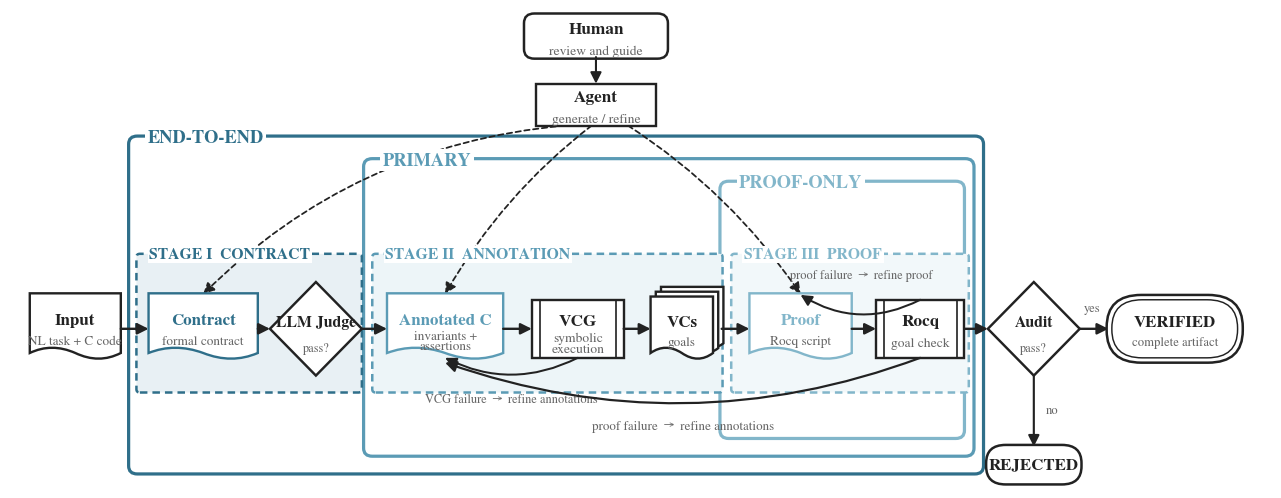
\includegraphics[width=0.94\textwidth]{figures/task_design_agentic.png}
\caption{The \textsc{CAV-Bench} construction and evaluation pipeline.}
\label{fig:task-design}
\end{figure*}

Figure~\ref{fig:task-design} summarizes the workflow. The primary task fixes the contract and evaluates the auxiliary annotation and proof stages. We additionally provide an end-to-end task that evaluates all three stages and a proof-only task that supplies the contract and auxiliary annotations to isolate the proof stage. Across all tasks, a deterministic audit checks the submitted artifacts and decides success rather than relying on the agent's own claim.

We conduct extensive experiments across frontier code-agent and model configurations and multiple reasoning-effort levels. Even the strongest evaluated configuration, Codex with GPT-5.5 at xhigh effort, verifies only 57.1\% of the 140 primary-task instances within the 90-minute budget. Accepted runs still require tens of minutes, millions of input tokens, and repeated repository and checker interaction. These results leave substantial room to improve not only verification accuracy, but also trajectory efficiency, stopping behavior, and time and token cost.

Our contributions are:
\begin{itemize}
    \item \textbf{A HumanEval benchmark for formal C verification:} 140 tasks pairing natural-language problem descriptions with executable C implementations (adapted from C++ as no C version existed) and their formal  contracts. Verification revealed discrepancies in several original solutions.
    \item \textbf{Human-in-the-loop construction of fully verified ground truth:} experts guide a code agent to produce complete auxiliary annotations and Rocq proofs, all checked by a deterministic audit.
    \item \textbf{Three agent tasks with experimental baselines:} contract-to-proof, end-to-end, and proof-only tasks, plus large-scale measurements of yield, reasoning effort, stage coupling, termination failures, and tool-use iteration.
\end{itemize}

\section{Preliminaries}
\label{sec:preliminaries}

\paragraph{Program verification.}
Program verification formally checks whether an implementation satisfies its contract.  Contract gives pre- and post-conditions specifying the intended behavior. Auxiliary annotations, notably loop invariants,  supply intermediate facts  bridging the precondition to the postcondition. A verification condition generator (VCG) then performs program reasoning on the implementation, contract, and annotations to produce proof obligations, purely logical formulas independent of control flow.  Proof discharges these obligations using a proof assistant. 
 If all pass, verification succeeds; if not, it may require repairing the proof or strengthening the annotation, after which the VCG is rerun.
 %A failed goal may require repairing the Proof or strengthening the Auxiliary Annotation.

\paragraph{QCP.}

QCP~\cite{wu2025qcppracticalseparationlogicbased} is the verification environment we use throughout this work. It is a separation logic-based verifier for C, able to describe memory layouts and changes.   Given an implementation, contract, and annotations, QCP invokes its VCG to generate proof obligations in separation logic, which are then discharged in Rocq, where VCG and proof checking are integrated. This unified loop provides deterministic feedback, VCG errors or proof failures supporting iterative revision across stages.

%QCP is a separation-logic-based C verification tool that can describe memory ownership and changes~\cite{wu2025qcppracticalseparationlogicbased}. Given an implementation, Contract, and Auxiliary Annotation, it runs VCG and uses Rocq to check the Proof. Its feedback supports repeated refinement of Auxiliary Annotation and Proof.

\paragraph{Example.}
HumanEval Problem 52, \texttt{below\_threshold}, returns whether every array element is below \texttt{t}. 
The contract specifies functional correctness (via predicates \texttt{pre}, \texttt{post}) and memory safety via \texttt{IntArray::full}. The annotation provides a loop invariant. The VCG generates proof obligations: the invariant must hold on entry, be preserved by each iteration, and imply the postcondition on exit. The proof discharges them in Rocq.
\begin{lstlisting}[style=artifactvscode,basicstyle=\ttfamily\fontsize{5.2}{5.7}\selectfont,aboveskip=2pt,belowskip=2pt,escapeinside={(*!}{!*)}]
int p052_below_threshold(int *l, int l_size, int t)
(*!\codebadge{stagecontractcolor}{CONTRACT}!*)
(*!\stagecodeline{stagecontractcolor}{/*@ With xs}!*)
(*!\stagecodeline{stagecontractcolor}{ Require 0 <= l_size && l_size < INT_MAX && pre(xs) &&}!*)
(*!\stagecodeline{stagecontractcolor}{         IntArray::full(l, l_size, xs)}!*)
(*!\stagecodeline{stagecontractcolor}{ Ensure ((__return != 0) && post(xs,t,true) ||}!*)
(*!\stagecodeline{stagecontractcolor}{         (__return == 0) && post(xs,t,false)) &&}!*)
(*!\stagecodeline{stagecontractcolor}{         IntArray::full(l, l_size, xs) */}!*)
{
(*!\codebadge{stageannotationcolor}{AUXILIARY ANNOTATION}!*)
(*!\stagecodeline{stageannotationcolor}{  /*@ Inv Assert 0 <= i && i <= l_size && pre(xs) &&}!*)
(*!\stagecodeline{stageannotationcolor}{      (forall (k: Z), (0 <= k && k < i) => Znth(k,xs,0) < t) &&}!*)
(*!\stagecodeline{stageannotationcolor}{      IntArray::full(l, l_size, xs) */}!*)
  for (i = 0; i < l_size; i++)
    if (l[i] >= t) return 0;
  return 1;
}

(*!\codebadge{stageproofcolor}{PROOF (EXCERPT)}!*) (*!\stagecodeline{stageproofcolor}{Proof. pre_process; ...; lia. Qed.}!*)
\end{lstlisting}

\section{Related Work}
\label{sec:related-work}

\paragraph{Code-generation benchmarks.}
Function-level benchmarks such as HumanEval, MBPP, APPS, and CodeContests usually evaluate generated programs through tests~\cite{chen2021evaluating,austin2021program,hendrycks2021apps,li2022alphacode}. MultiPL-E, ClassEval, LiveCodeBench, and BigCodeBench extend coverage across languages, program structures, time, and realistic library use~\cite{cassano2022multiple,du2025classeval,jain2025livecodebench,zhuo2025bigcodebench}. RepoBench adds repository context, while SWE-agent, SWE-bench, SWE-Bench Pro, and Terminal-Bench evaluate tool-using agents on repository or command-line tasks~\cite{liu2024repobench,yang2024sweagent,jimenez2024swebench,deng2026swebenchpro,merrill2026terminalbench}. \textsc{CAV-Bench} adopts this repository interaction setting but asks agents to formally verify a fixed C implementation rather than generate or repair code.

\paragraph{Theorem-proving benchmarks.}
Recent mathematical theorem-proving benchmarks are centered largely on Lean. MiniF2F and FIMO formalize Olympiad-level problems, ProofNet targets undergraduate mathematics, and PutnamBench extends competition mathematics across Lean, Isabelle, and Coq~\cite{zheng2021minif2f,liu2023fimo,azerbayev2023proofnet,tsoukalas2024putnambench}. CoqGym and CoqStoq instead evaluate proof synthesis across open-source Coq projects, with CoqStoq introduced alongside Rango~\cite{yang2019learning,thompson2025rango}. These benchmarks evaluate theorem or proof-state completion rather than a verification workflow rooted in executable programs that couples auxiliary annotations with proofs.

\paragraph{Program-verification benchmarks.}
Program-verification benchmarks cover complementary parts of the workflow. FormalBench, \textsc{Coins}, and specification-inference work emphasize contracts or semantic properties, while InvBench focuses on auxiliary annotations~\cite{cosler2023nl2spec,autospec,ma2025specgen,lecong2025formalbench,yang2026coins,wei2025invbench}. DafnyBench, CloverBench, CLEVER, VERINA, VeriBench, VeriEquivBench, Vericoding, AlgoVeri, and VeriContest study broader combinations of verifiable code and proofs, while FVAPPS, NTP4VC, and VeriSoftBench emphasize proofs or proof repositories~\cite{loughridge2024dafnybench,sun2024clover,thakur2025clever,ye2026verina,miranda2026veribench,zeng2026veriequivbench,bursuc2025vericoding,zhao2026algoveri,xie2026vericontest,dougherty2025proving,xu2026neural,xin2026verisoftbench}. These benchmarks do not evaluate the coupled auxiliary-annotation and proof workflow for C programs, where auxiliary annotations must explicitly characterize memory.

\paragraph{C program verification.}
Many tools have been developed for C program verification, using different Contract languages and proof workflows. Frama-C uses ACSL to express quantified conditions, program behaviors, and memory changes, and its WP plugin relies mainly on automated provers~\cite{kirchner2015framac}. VeriFast instead uses separation logic to express memory ownership and recursive data structures, which it checks through symbolic execution~\cite{jacobs2011verifast}. QCP combines memory-aware Contracts and Rocq definitions with an explicit Rocq Proof, exposing the interaction between Auxiliary Annotation and Proof that \textsc{CAV-Bench} evaluates~\cite{wu2025qcppracticalseparationlogicbased}.



\begin{table*}[t]
\centering
\scriptsize
\setlength{\tabcolsep}{3.2pt}
\caption{Comparison with program-verification benchmarks. Filled marks indicate components generated and evaluated in the benchmark; ``GT Verified'' indicates that the complete ground-truth artifact passes the corresponding checker.}
\label{tab:related-work-comparison}
\begin{tabular}{L{0.145\textwidth}L{0.185\textwidth}ccccc}
\toprule
\rowcolor{benchmarkhead}
Benchmark & Language / verifier & Spec. & Inv. & Other Ann. & ITP proof & GT Verified \\
\midrule
FormalBench & Java / OpenJML & \benchyes & \benchyes & \benchyes & \benchno & \benchno \\
InvBench & C / UAutomizer & \benchno & \benchyes & \benchno & \benchno & \benchno \\
DafnyBench & Dafny & \benchno & \benchno & \benchyes & \benchno & \benchyes \\
CloverBench & Dafny & \benchyes & \benchyes & \benchyes & \benchno & \benchyes \\
CLEVER & Lean & \benchyes & \benchno & \benchno & \benchyes & \benchno \\
VERINA & Lean & \benchyes & \benchno & \benchno & \benchyes & \benchno \\
VeriBench & Lean & \benchyes & \benchno & \benchno & \benchyes & \benchno \\
AlgoVeri & Dafny / Verus / Lean & \benchno & \benchyes & \benchyes & \benchyes & \benchno \\
FVAPPS & Lean & \benchno & \benchno & \benchno & \benchyes & \benchno \\
NTP4VC & Lean / Rocq / Isabelle & \benchno & \benchno & \benchno & \benchyes & \benchyes \\
VeriSoftBench & Lean & \benchno & \benchno & \benchno & \benchyes & \benchyes \\
\rowcolor{benchmarkhighlight}
\textsc{CAV-Bench} & C / Rocq & \benchyes & \benchyes & \benchyes & \benchyes & \benchyes \\
\bottomrule
\end{tabular}
\end{table*}

Table~\ref{tab:related-work-comparison} summarizes this comparison. Unlike the compared benchmarks, \textsc{CAV-Bench} requires a repository-running agent to complete the coupled auxiliary annotation and proof workflow for a fixed C implementation and contract.

\section{CAV-Bench}
\label{sec:benchmark-design}

\textsc{CAV-Bench} turns HumanEval programs and their contracts into 140 repository-level C verification tasks. We construct the benchmark by collecting and adapting the source materials, building verified ground truth, and defining three task settings.

\subsection{Benchmark Data Collection}

Each \textsc{CAV-Bench} task is built from a natural language description and a C implementation, together with a complete ground-truth artifact consisting of a QCP contract, auxiliary annotations, and Rocq proofs. \wslcomment{The descriptions come from HumanEval~\cite{chen2021evaluating}, and the C implementations are  adapted from the corresponding C++ implementations in HumanEval-X~\cite{zheng2023codegeex}, with modifications to accommodate C's  data representation, library operations, and memory management. During verification of the adapted C implementations,  we found several cases whose behavior deviated  from the original HumanEval descriptions. We corrected the implementations to match the descriptions and report the affected tasks in the supplementary material. For contracts, we adapt the human-written Rocq contracts released with \textsc{Coins}~\cite{yang2026coins} (which specify functional correctness only) into QCP contracts, adding  conditions to establish memory safety and the absence of runtime errors (RTEs) in C. We also retain or adapt any mathematical helper definitions required by the contracts.}

Of the 164 HumanEval problems, 140 enter \textsc{CAV-Bench}. We mainly exclude floating-point programs because their numerical reasoning is beyond the practical scope of the current QCP workflow.

\begin{table}[t]
\centering
\scriptsize
\setlength{\tabcolsep}{4pt}
\caption{Statistics of the verified \textsc{CAV-Bench} corpus.}
\label{tab:benchmark-components}
\begin{tabular}{L{0.50\columnwidth}rr}
\toprule
\rowcolor{benchmarkhead}
Statistic & Total & Mean / task \\
\midrule
HumanEval source problems & 164 & -- \\
Verified benchmark problems & 140 & -- \\
C code LOC & 4,076 & 29.1 \\
Function-contract LOC & 3,114 & 22.2 \\
Auxiliary-annotation LOC & 10,270 & 73.4 \\
Task-specific Rocq definition LOC & 8,083 & 57.7 \\
Manual Rocq proof LOC & 62,812 & 448.7 \\
Generated verification conditions & 5,562 & 39.7 \\
\bottomrule
\end{tabular}
\end{table}

% Each task is built from a fixed C implementation, its natural-language description, a QCP contract, and any required Rocq definitions. Agents work in the QCP repository, where they can run VCG and Rocq, read the documentation and examples, and import the provided Rocq libraries in their proofs. Ground-truth auxiliary annotations and proofs are revealed only when required by the task setting.

Agents work in the QCP repository, where they can run the VCG and Rocq, consult documentation and examples, and import
the provided Rocq libraries. The QCP contract with required Rocq definitions, and auxiliary annotations are exposed only when
required by the task setting. Ground-truth Rocq proofs are never exposed to agents.

\subsection{Ground-Truth Construction}
\label{sec:human-loop-workflow}

We construct a complete verification result for every included problem through the human-agent workflow in Figure~\ref{fig:task-design}. \wslcomment{Starting from a C implementation and the contract derived from \textsc{Coins}}, human experts guide a code agent to produce auxiliary annotations and proof. QCP's VCG analyzes the annotated C program and generates proof goals, which Rocq then checks~\cite{wu2025qcppracticalseparationlogicbased}. The agent iteratively revises the auxiliary annotations and proof based on feedback from these tools.

Human experts review intermediate results, provide semantic guidance when the agent stalls, and check the final contract against the HumanEval description and the adapted \textsc{Coins} contract. \wslcomment{They prevent the agent  from using commands that bypass proof obligations (e.g., \texttt{admit} or \texttt{axiom}), but do not write task-specific proofs or annotations themselves.}

A task is included only when rerunning VCG regenerates all proof goals, Rocq accepts every proof, and the experts confirm that the contract preserves the intended behavior. %Programs beyond the current capabilities of QCP and results that do not pass these checks are excluded. 
Because this construction process includes human effort that is not fully recorded, its time and token costs are not directly comparable with the fully automated evaluation runs.

\subsection{Task Design}

The 140 verified results define the three task settings shown in Figure~\ref{fig:task-design}. Our primary \emph{contract-to-proof} task provides a fixed, human-reviewed, \wslcomment{formally verified ground-truth contract} and asks the agent to complete the auxiliary annotation and proof stages. Fixing the contract gives every agent the same intended behavior while focusing on the interaction between auxiliary annotations and proofs.

We additionally provide two tasks. The \emph{end-to-end} task asks the agent to complete all three stages. Because different contracts may correctly describe the same behavior, contract quality cannot be determined by a single automatic check. We therefore use a lightweight rubric to evaluate whether the generated contract adequately covers the intended behavior and safety requirements, with details provided in the supplementary material. The \emph{proof-only} task supplies the  contract and the ground-truth auxiliary annotations, allowing us to evaluate proof construction separately.

Evaluated agents receive no expert guidance or task-specific proof hints. The deterministic audit reruns VCG and Rocq, checks that the fixed contract and executable implementation remain unchanged, detects ways of avoiding the required proof, and verifies that the agent did not read disallowed material. Further details are provided in the supplementary material.

\providecommand{\nontimeoutcost}[1]{%
  \begingroup\setlength{\fboxsep}{0.7pt}\colorbox{gray!15}{\strut #1}\endgroup}
\begin{table*}[!t]
\centering
\caption{Primary-task results over 140 tasks. Missing runs are counted as timeouts. Each cost cell reports the audited-success mean followed by the gray non-timeout mean, which includes failed submissions. Operation counts include only recorded trace events, and rounds count assistant messages.}
\label{tab:main_results}
\scriptsize
\setlength{\tabcolsep}{3.0pt}
\renewcommand{\arraystretch}{1.04}
\resizebox{\textwidth}{!}{%
\begin{tabular}{lrrr|rr|rrrr}
\toprule
\rowcolor{gray!15}
& \multicolumn{3}{c|}{Outcome} & \multicolumn{2}{c|}{Cost} & \multicolumn{4}{c}{Trace activity} \\
\rowcolor{gray!15}
Model / effort & $W/140$ & $F/T$ & SR (\%) & Time (min) & In (M) / Out (k) & Read / Write & Tools & Rocq / VCG & Rounds \\
\midrule
\textit{Codex} & & & & & & & & & \\
\quad GPT-5.5 (xhigh) & 80/140 & 31/29 & \textbf{57.1} & 42.8\,\nontimeoutcost{45.1} & 9.1/35\,\nontimeoutcost{9.9/38} & 79.9/7.1\,\nontimeoutcost{81.6/9.0} & 119.7\,\nontimeoutcost{125.3} & 12.6/3.0\,\nontimeoutcost{14.5/3.6} & 55.8\,\nontimeoutcost{59.7} \\
\quad GPT-5.5 (medium) & 59/140 & 61/20 & 42.1 & 33.4\,\nontimeoutcost{36.6} & 7.0/23\,\nontimeoutcost{9.8/30} & 65.5/8.1\,\nontimeoutcost{71.0/14.6} & 99.0\,\nontimeoutcost{116.5} & 11.0/3.3\,\nontimeoutcost{18.4/4.0} & 49.3\,\nontimeoutcost{63.8} \\
\quad GPT-5.4 (xhigh) & 53/140 & 48/39 & 37.9 & 38.5\,\nontimeoutcost{45.8} & 22.4/78\,\nontimeoutcost{24.6/85} & 94.3/25.5\,\nontimeoutcost{109.2/33.7} & 171.0\,\nontimeoutcost{200.5} & 43.1/3.0\,\nontimeoutcost{48.8/4.8} & 49.5\,\nontimeoutcost{58.8} \\
\quad GPT-5.4 (high) & 40/140 & 96/4 & 28.6 & 43.1\,\nontimeoutcost{39.5} & 20.3/59\,\nontimeoutcost{21.8/67} & 95.8/35.8\,\nontimeoutcost{101.1/36.2} & 156.3\,\nontimeoutcost{169.4} & 31.4/2.2\,\nontimeoutcost{32.9/4.9} & 52.1\,\nontimeoutcost{47.7} \\
\quad GPT-5.4 (medium) & 20/140 & 120/0 & 14.3 & 21.2\,\nontimeoutcost{23.9} & 15.1/41\,\nontimeoutcost{15.2/47} & 66.0/30.6\,\nontimeoutcost{77.4/29.0} & 125.1\,\nontimeoutcost{132.9} & 33.8/2.5\,\nontimeoutcost{27.8/5.4} & 31.9\,\nontimeoutcost{36.2} \\
\quad GPT-5.4 (low) & 16/140 & 124/0 & 11.4 & 21.7\,\nontimeoutcost{16.2} & 14.7/36\,\nontimeoutcost{10.3/31} & 59.3/29.4\,\nontimeoutcost{57.3/20.6} & 125.8\,\nontimeoutcost{103.6} & 34.6/2.8\,\nontimeoutcost{18.9/5.0} & 29.7\,\nontimeoutcost{26.6} \\
\quad GPT-5.4-mini (medium) & 8/140 & 130/2 & 5.7 & 36.4\,\nontimeoutcost{38.4} & 18.7/103\,\nontimeoutcost{19.2/111} & 89.4/36.0\,\nontimeoutcost{102.4/33.6} & 171.2\,\nontimeoutcost{181.7} & 45.6/2.0\,\nontimeoutcost{35.2/9.5} & 81.1\,\nontimeoutcost{95.6} \\
\addlinespace[2.2pt]
\textit{Claude Code} & & & & & & & & & \\
\quad GLM-5.2 (thinking) & 30/140 & 77/33 & 21.4 & 28.3\,\nontimeoutcost{48.6} & 11.5/93\,\nontimeoutcost{15.4/105} & 79.5/27.1\,\nontimeoutcost{119.8/39.2} & 105.8\,\nontimeoutcost{151.9} & 31.0/3.3\,\nontimeoutcost{44.2/6.5} & 89.8\,\nontimeoutcost{136.3} \\
\quad DeepSeek-V4-Pro (thinking) & 5/140 & 55/80 & 3.6 & 33.2\,\nontimeoutcost{69.8} & 14.5/73\,\nontimeoutcost{27.4/69} & 81.0/50.8\,\nontimeoutcost{100.4/54.2} & 142.6\,\nontimeoutcost{175.2} & 46.4/5.0\,\nontimeoutcost{43.6/14.5} & 130.0\,\nontimeoutcost{149.2} \\
\addlinespace[2.2pt]
\textit{Kimi Code} & & & & & & & & & \\
\quad kimi-2.7-code (thinking) & 18/140 & 99/23 & 12.9 & 38.8\,\nontimeoutcost{64.8} & 17.0/86\,\nontimeoutcost{30.3/147} & 114.1/42.5\,\nontimeoutcost{185.8/88.5} & 166.3\,\nontimeoutcost{274.6} & 44.5/3.6\,\nontimeoutcost{86.6/9.9} & 157.6\,\nontimeoutcost{264.8} \\
\bottomrule

\end{tabular}%
}
\end{table*}

\begin{figure*}[!t]
    \centering
    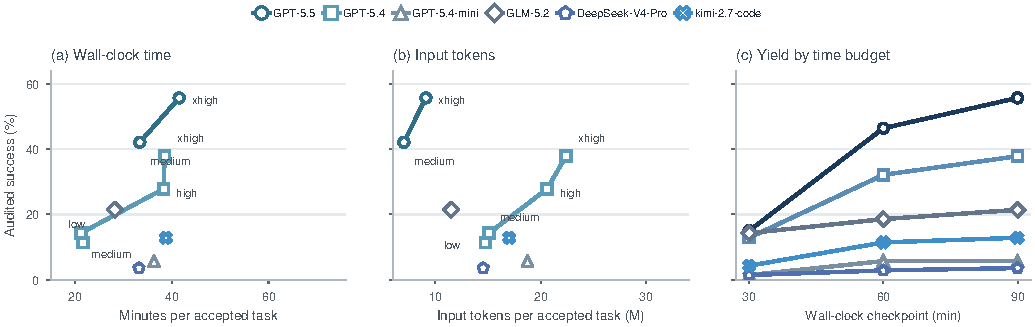
\includegraphics[width=0.91\textwidth]{figures/effort_scaling.pdf}
    \caption{Success and successful-run cost across models and reasoning-effort levels. Color and marker shape jointly identify each model. Panels (a) and (b) plot audited success against mean wall-clock time and input tokens per accepted task; connected points vary reasoning effort within a GPT model family. Panel (c) reports cumulative audited success at 30, 60, and 90 minutes using the strongest GPT effort level and the fixed configuration of each other model.}
    \label{fig:rq4_reasoning}
\end{figure*}

\section{Experiments and Results}
\label{sec:experiments}

\paragraph{Experimental setup.}
We evaluate code agents on the primary contract-to-proof task across all 140 tasks. Each agent receives a fixed C implementation and contract and works in the QCP repository to complete the auxiliary annotations and proof. All agents receive the same general workflow guidance and may use VCG, Rocq, the provided documentation and examples, and the Rocq libraries, but receive no task-specific hints. Each run has a 90-minute wall-clock budget. A deterministic audit decides success by rerunning VCG and Rocq and checking the submitted artifact as described.

For each model and reasoning-effort configuration, we report audited successes ($W$), non-timeout failures ($F$), and timeouts ($T$), conservatively counting missing runs as timeouts. An audited completion counts as a success only if its recorded end-to-end wall-clock time is at most 5,400 seconds; audited completions exceeding this limit are counted as timeouts. Every success rate uses all 140 tasks as its denominator. In each cost cell of Table~\ref{tab:main_results}, the first value averages over successful runs and the gray value averages over all non-timeout runs, including failed attempts. We use a model's official harness when available and Claude Code otherwise; RQ5 studies the effect of harness choice.

\subsection{RQ1: How Well Do Code Agents Complete C Verification?}
Table~\ref{tab:main_results} shows that the strongest configuration, GPT-5.5 at xhigh effort, verifies only 80 of the 140 tasks (57.1\%) within 90 minutes. Even these short HumanEval-derived functions require repeated repository exploration, auxiliary-annotation revisions, proof repairs, and VCG and Rocq checks. Figure~\ref{fig:rq4_reasoning}(c) shows that audited success continues to increase from 30 to 60 and 90 minutes for the strongest configurations, confirming that formal verification requires long-horizon interaction. However, additional time alone is insufficient. Many agents stop before timeout without producing an accepted result, showing that they often fail to recognize when verification remains incomplete. We should use deterministic loop engineering to make termination depend on external verification rather than model judgment. The interaction counts in Table~\ref{tab:main_results} further confirm that success requires sustained repository work, while the gray values show that failed runs can remain expensive.
% \finding{Even short functions require long-horizon verification, and many agents stop before the submitted artifact passes the audit.}

\finding{Even short C functions require long-horizon verification: the strongest configuration solves only 57.1\% of tasks within 90 minutes, and many agents terminate before the timeout without passing the external audit.}

\subsection{RQ2: How Do Capability and Reasoning Effort Affect Performance?}
Figure~\ref{fig:rq4_reasoning} and the trace columns of Table~\ref{tab:main_results} reveal a joint capability--effort scaling pattern. Greater model capability generally reduces the time, token demand, tool use, and exploratory work needed to reach an accepted solution, whereas increasing reasoning effort within a model sustains longer trajectories and raises local inference cost. Overall, higher reasoning effort tends to increase resource use, but fewer unproductive steps partially offset the added inference cost. Reasoning effort also controls persistence. Low-effort configurations disproportionately terminate before the wall-clock limit, while higher effort keeps the agent working through checker failures and repository revisions. Thus, effort changes not only the quality of individual decisions but also whether the agent continues an unresolved task long enough to solve it.
% \finding{Capability makes agent trajectories more efficient, while reasoning effort increases persistence and resource investment; their marginal cost diminishes as stronger reasoning eliminates unproductive exploration.}
\finding{Greater capability makes agent trajectories more efficient, whereas greater reasoning effort increases persistence and resource use. However, the marginal resource cost of additional reasoning declines as stronger reasoning reduces unproductive exploration.}

\subsection{RQ3: Where Does Difficulty Arise Across Verification Stages?}
\begin{figure*}[!t]
    \centering
    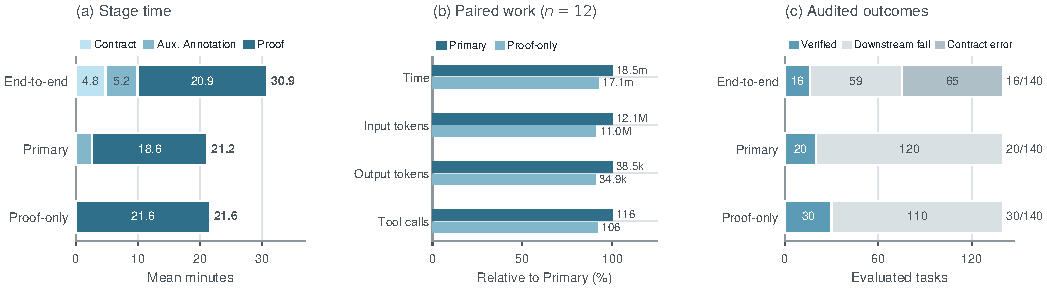
\includegraphics[width=\textwidth]{figures/branch_difficulty.pdf}
    \caption{Stage-level results for GPT-5.4 at medium effort. Panel (a) shows the mean time spent in each stage for accepted runs. Panel (b) compares cost on tasks accepted in both the primary and proof-only settings, with each metric normalized to the primary task. Panel (c) reports audited outcomes for the three task settings.}
    \label{fig:rq2_difficulty}
\end{figure*}
Figure~\ref{fig:rq2_difficulty} compares the three task settings using GPT-5.4 at medium effort. The proof stage takes most of the successful-run time, but much of its difficulty comes from the interaction between auxiliary annotations and proofs. Missing or incorrect auxiliary annotations can produce proof goals that cannot be proved, while proof failures often reveal which facts must be added to the auxiliary annotations. Supplying verified auxiliary annotations in the proof-only task improves success from 20 to 30 tasks. Among the 12 tasks accepted in both settings, it also reduces time, input tokens, output tokens, and tool calls.

The contract stage requires less runtime but is difficult to evaluate. Different contracts may correctly describe the same behavior, and an automatically accepted contract may still be too weak or fail to capture the intended behavior. The agent therefore lacks the deterministic feedback available in the auxiliary annotation and proof stages, and many generated contracts are rejected before reaching the later stages.
\finding{Proof takes most of the runtime, but the interaction between  auxiliary annotations and proofs  drives much of the difficulty; contract generation remains hard because it lacks deterministic feedback.}

\subsection{RQ4: Why Do Agent Runs Fail?}
\begin{table}[t]
    \centering
    \caption{Primary-task failures by model configuration. Categories may overlap. $F/T$ denotes non-timeout failures/timeouts, with missing runs counted as timeouts; $P/I/R$ denotes invalid proofs, fixed-input modifications, and reads of disallowed material.}
    \label{tab:error_analysis_models}
    \scriptsize
    \setlength{\tabcolsep}{3.2pt}
    \renewcommand{\arraystretch}{1.02}
    \begin{tabular}{@{}lccc@{}}
        \toprule
        \rowcolor{benchmarkhead}
        & Outcome & Stage & Audit \\
        \rowcolor{benchmarkhead}
        Model / effort & $F/T$ & Proof/VCG & $P/I/R$ \\
        \midrule
        \textit{Codex} & & & \\
\quad GPT-5.5 (xhigh) & 31/31 & 29/2 & 7/13/5 \\
\quad GPT-5.5 (medium) & 61/20 & 57/4 & 11/19/7 \\
\quad GPT-5.4 (xhigh) & 48/39 & 44/4 & 6/29/16 \\
\quad GPT-5.4 (high) & 96/5 & 91/5 & 6/12/28 \\
\quad GPT-5.4 (medium) & 120/0 & 110/10 & 9/14/28 \\
\quad GPT-5.4 (low) & 124/0 & 102/22 & 3/18/33 \\
\quad GPT-5.4-mini (medium) & 130/2 & 96/34 & 0/33/86 \\
\addlinespace[2.2pt]
\textit{Claude Code} & & & \\
\quad GLM-5.2 (thinking) & 77/33 & 73/4 & 1/9/55 \\
\quad DeepSeek-V4-Pro (thinking) & 55/80 & 46/9 & 0/17/39 \\
\addlinespace[2.2pt]
\textit{Kimi Code} & & & \\
\quad kimi-2.7-code (thinking) & 99/23 & 96/3 & 5/21/92 \\
\midrule
\textbf{Total} & \textbf{841/233} & \textbf{744/97} & \textbf{48/185/389} \\
\bottomrule

    \end{tabular}
\end{table}
% Table~\ref{tab:error_analysis_models} reports failure categories that may overlap. A run is counted as a VCG failure when VCG produces no proof goals; otherwise, an unsuccessful run is counted as a proof failure. Audit failures are counted separately.

% Of the 841 non-timeout failures, 744 (88.5\%) occur after proof goals are generated, while 97 (11.5\%) fail at VCG. GPT-5.4-mini and GPT-5.4 at low effort have the most VCG failures, while Kimi-2.7-code and GPT-5.4-mini most frequently read disallowed material.

% Audit failures are separate from verification-stage failures. They include bypassing the required proof, modifying the fixed contract or implementation, and reading disallowed material. Their frequency shows that instructions and model-reported completion are insufficient; success must be determined by a deterministic audit.
% \finding{Most failures reach the proof stage, while frequent audit violations show that deterministic audit is necessary.}

Table~\ref{tab:error_analysis_models} reports failure categories that may overlap. We classify a run as a VCG-stage failure
when VCG produces no proof goals. Otherwise, we classify it as reaching the proof stage. Audit failures are counted separately.

Of the 841 non-timeout failures, 744 (88.5\%) reach the proof stage, while 97 (11.5\%) fail at VCG. GPT-5.4-mini and GPT-5.4
at low effort have the most VCG failures, while Kimi-2.7-code and GPT-5.4-mini most frequently read disallowed material. The predominance of proof-stage failures indicates that most difficulties arise after proof obligations are generated. However, because annotations shape these obligations, the category may capture failures in both annotation construction and proof writing.

Audit failures are separate from verification-stage failures. They include bypassing the required proof, modifying the fixed
contract or implementation, and reading disallowed material. Their frequency shows that instructions and model-reported
completion are insufficient; success must be determined by a deterministic audit.


\finding{Most failures reach the proof stage, highlighting the interaction between auxiliary annotations and proofs; frequent audit violations make deterministic auditing necessary.}



\subsection{RQ5: How Does the Agent Harness Affect Performance?}
\label{sec:harness-effects}

A harness gives the model repository access, runs tool commands, and manages context. The main experiments use Claude Code for GLM-5.2. We take all 30 tasks that GLM-5.2 completes under Claude Code and rerun the same model on them through OpenCode and Codex CLI. This cohort is fixed before inspecting either alternative harness. The implementation, contract, repository, instructions, 90-minute budget, and deterministic audit remain unchanged. The comparison therefore measures how many Claude Code successes each harness retains, rather than ranking the harnesses over all 140 tasks.

\begin{figure*}[!t]
\centering
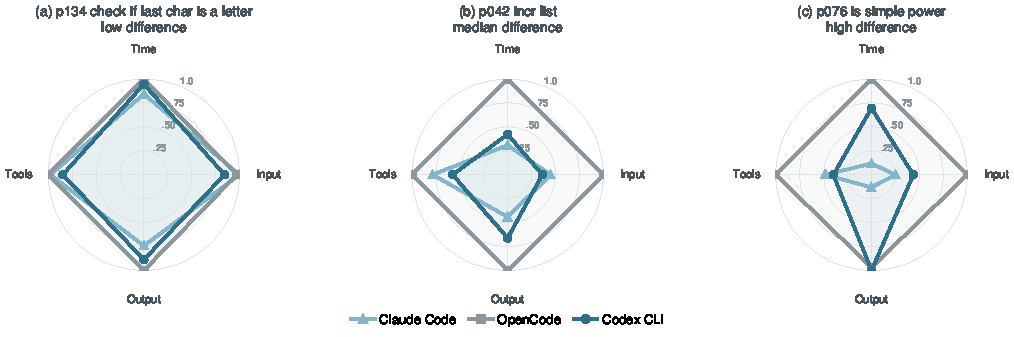
\includegraphics[width=0.86\textwidth]{figures/harness_task_radars.pdf}
\caption{Cost profiles for three GLM-5.2 tasks accepted under all three harnesses, chosen to represent low, median, and high cross-harness differences. Each metric is normalized to the largest value for that task, so smaller values indicate lower cost.}
\label{fig:harness-sensitivity}
\end{figure*}

Claude Code accepts 30/30 tasks by construction. Codex CLI retains 23 successes (76.7\%), while OpenCode retains 13 (43.3\%). Codex CLI has three timeouts and OpenCode has eleven. Changing only the harness can therefore cause the same model to lose previously successful tasks and can change whether an unsuccessful run stops early or uses the full budget.

The harnesses solve different tasks, so their mean cost over all successes is not directly comparable. We instead compare the 12 tasks solved by all three. On this shared set, Claude Code uses the least time, tokens, and tool calls. Codex CLI retains more of the original cohort than OpenCode, but costs more than Claude Code on the shared tasks; OpenCode costs the most. Figure~\ref{fig:harness-sensitivity} further shows that cross-harness cost can be nearly identical on one task but differ sharply on another. Harness choice is therefore part of the evaluated system, not merely a way to access the model.
\finding{Harness choice materially affects both acceptance and cost. Codex CLI performs relatively close to Claude Code, but no alternative harness recovers all Claude Code successes.}

\section{Limitations}
\label{sec:threats-validity}

\paragraph{Program scale.}
The 140 benchmark tasks are short, single-function HumanEval programs. They do not cover large APIs, concurrent systems, or multi-module verification projects, so the results may not generalize to larger and more complex programs. Nevertheless, formally verifying these programs remains extremely challenging even at this scale.

\paragraph{Model coverage.}
We evaluate a representative subset of models and effort configurations rather than all available systems. The observed accuracies and rankings should therefore not be extrapolated beyond the evaluated configurations.

\paragraph{Evaluation cost.}
At public list prices, the evaluated runs represent approximately \$6,700 in API-equivalent inference cost. Agentic verification involves long trajectories and repeated model calls, making evaluation expensive even for HumanEval-scale programs. This cost constrains both the scale of the programs and the number of model configurations that we can evaluate.

\section{Conclusion}

\textsc{CAV-Bench} provides 140 repository-level tasks for long-horizon C verification under QCP--Rocq. The strongest configuration verifies only 55.7\%, with failures across annotation construction, verification-condition generation, and Rocq proofs. Persistent capability and harness effects, together with frequent invalid artifacts, make C verification a rigorous benchmark for feedback-driven code agents and deterministic auditing.


\bibliography{references}

\end{document}
